\part{The back end}\label{part:nstar}


\chapter{Introduction}\label{chap:nstar-abstract}

Assembly languages are the lowest level of humanly-possible programming there exists nowadays. They were used back in the days for very performance-critical tasks, or even just for fun, as there weren't many other programming languages available. Nowadays, with all the existing ones, most people have never used any assembly language.

Despite their apparent simplicity, and the small amount of work you need to put into creating assembly languages, those are in fact very hard to use. At that low level, there is no such thing as Java's exceptions keeping you from doing dumb things, Rust's linear types keeping you from leaking memory nor even Garbage Collectors. The nice things preventing you from having segfaults simply do not exist, and you are expected to either provide all those things yourself (creating a language runtime) or be very careful about what you are doing each time you write a single instruction (even a simple \texttt{mov} can have undesirable side-effects).

Doing dumb things is something that we must prevent directly when using the language. That way, we do not need to rely on external verification tools or debuggers, trying to know why a program segfaults at a specific point.
This is where a type system can become handy. Typed assembly languages are assembly languages augmented with simple yet powerful type system. Among the most famous typed assembly languages are TALx86~\cite{TALx86} and DTAL~\cite{DTAL}.

TALx86 is basically NASM with a type system, targetting only the x86 architecture. DTAL is much more complicated and embeds a completely dependent type system.

\vspace{\baselineskip}

N*'s goal is to assist users with a simple but powerful type system, as well as other features like what I call ``branch-checking'' which prevents from leaking the control flow of the program, and thus makes a part of the type-checking process meaningful.
But before even being a usable programming language, N* aims at being a compiler backend (much like for example LLVM), and is used as is in the Zilch project. Differences with other compiler backends are mostly the type-system, allowing the compilation of Zilch source code into type-safe instructions.

\vspace{\baselineskip}

Because N* supports compiling to multiple architectures, using different grammars, describing N* will at first be platform-agnostic, treating common aspects between all CPU architectures, and then will be divided into multiple categories, explaining in more details some features on a per-architecture basis\footnote{Note that the target executable format (ELF, PE, \ldots) is also considered as an architecture-specific thing, but should not influence N* much.}.

\chapter{Non platform-specific features}\label{chap:nstar-common}

\section{Types}\label{sec:nstar-common-ts}

One of the differences between classical assembly languages and N* is its type system.
Compared to other higher level programming languages like Java, C++, etc, N* has a very simple yet powerful and expressive enough type system.

In programming, types are used mostly to prove at compile-time that a given program should behave well if it type-checks. While this works for more elaborated programming languages like Haskell, Idris, etc, most type systems aren't expressive enough to absolutely guarantee that everything will work at run-time (in fact, there is no possible way of doing this, because for example a memory allocation may fail, and this cannot be endorsed at compile-time). However, we can try to guarantee as much as possible.

N* doesn't try to solve this issue, because it would be really hard to target a dependently typed assembly language from a non-dependently typed programming language. But where all used assembly languages do not even consider types (only numbers, in fact), N* embeds a powerful type system used to remove the possibility of bugs (like incorrect structure addresses passed as a parameter function, or incoherent types in some instructions).

\subsection{Integer types}\label{subsec:nstar-common-ts-integer}

Numbers are the building block of any assembly language. Most of data manipulated is manipulated as numbers, e.g. addresses, characters, strings, enumerations, etc.
This is not the case in N*, where ``integer''  only really means ``number''.
The syntax for the types of integers is given in Figure~\ref{fig:nstar-common-ts-integer-syntax}.

\begin{figure}[htb]
  \centering
  \scalebox{.5}{
    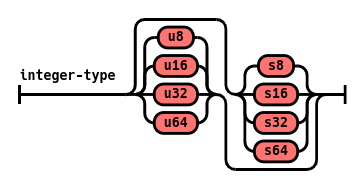
\includegraphics{nstar-integers-types-syntax}
  }
  \caption{Grammar for integer types.}
  \label{fig:nstar-common-ts-integer-syntax}
\end{figure}

Integers have two varying parameters: their sign and sizes.
According to the sign (i.e. signed or unsigned), some operations may not perform the same (for example \texttt{mul} does not behave the same).
The size is nothing more than the number of bits occupied by the integer (in N*, those are restricted to multiples of $8$ smaller or equal to $64$).
Most operations should perform the same no matter the integer size, however it is recommended to search in the target architecture manual for further reference.

\subsection{Other atomic types}\label{subsec:nstar-common-ts-otheratomic}

There are two other atomic types that we did not talk about, but refered to in the introduction of the type system: characters and pointers. Their respective syntax is given in Figure~\ref{fig:nstar-common-ts-atomic-syntax}.

In all assembly languages, characters are merely syntactic sugar for their ASCII code. This is how their are put in the machine code anyway, so it is not a huge problem (it might even not be at all).

Pointers, on the other hand, are unabstracted memory addresses.
In N*, there are two types of pointers: data pointers and stack pointers.
Stack pointers are covered in Subsection~\ref{subsec:nstar-common-ts-stack}~``\nameref{subsec:nstar-common-ts-stack}''.
Data pointers simply represent an address where we know (or not, see the Subsection~\ref{subsec:nstar-common-unsafe-derefliteraladdr}~``\nameref{subsec:nstar-common-unsafe-derefliteraladdr}'') that there is a value of the given pointed type.

They support two common operations: offsetting (see the Subsection~\ref{subsec:nstar-common-unsafe-ptroffset}~``\nameref{subsec:nstar-common-unsafe-ptroffset}'') and dereferencing (taking the value pointed by the pointer).
Dereferencing is considered a safe operation, unless trying to on a literal address.
There is no notion of ``null'' pointers, like \texttt{NULL} in C.
However, it is possible to use the literal \texttt{\$0} (which represents a pointer to the address $0$).

\begin{figure}[htb]
  \centering
  \scalebox{.5}{
    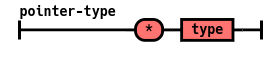
\includegraphics{nstar-ptr-type-syntax}
  } \\
  \scalebox{.5}{
    
\includegraphics{nstar-char-type-syntax}
  }
  \caption{Grammar for character and pointer types}
  \label{fig:nstar-common-ts-atomic-syntax}
\end{figure}

\subsection{Context types}\label{subsec:nstar-common-ts-records}

Record types (or contexts) are mappings from registers to types.
They are used to indicate that a register is bound to a value of a given type at a certain point in the program.
The grammar is described in Figure~\ref{fig:nstar-common-ts-records-syntax}.

\begin{figure}[htb]
  \centering
  \scalebox{.5}{
    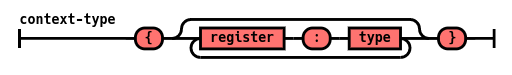
\includegraphics{nstar-records-syntax}
  }
  \caption{Grammar for context types.}
  \label{fig:nstar-common-ts-records-syntax}
\end{figure}

Context types are used to represent data contexts where any mapping is some sort of a proof that some data of some type is accessible through some register.

\vspace{\baselineskip}

\textbf{Note:} In the context of label types, a context type can be augmented by a \texttt{forall} generic type variable binder.
The grammar is described in Figure~\ref{fig:nstar-common-ts-label-types-syntax}.
The type variable binder is used to abstract away some details of the type through an opaque variable specialized at the call site.

\begin{figure}[htb]
  \centering
  \scalebox{.5}{
    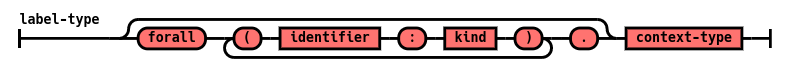
\includegraphics{nstar-label-types-syntax}
  }
  \caption{Grammar for label context types.}
  \label{fig:nstar-common-ts-label-types-syntax}
\end{figure}

The example code given in Listing~\ref{lst:nstar-common-ts-records-stackmask} shows a use for type variables.
The stack is abstracted away, meaning that we can call this function from anywhere, given any stack (as long as it is \texttt{call}ed, or \texttt{jmp}ed to from a \texttt{call}ed function).
The type variable \texttt{s} is specialized at the call site.

\begin{listing}[htb]
  \centering
  \begin{minipage}{0.80\textwidth}
    \begin{minted}[]{\nstarlexer}
      label: forall (s: Ts). { %rsp: sptr *{ %rsp: sptr s }::s }
          ret
    \end{minted}
  \end{minipage}
  \caption{Stack masking using a type variable binder.}
  \label{lst:nstar-common-ts-records-stackmask}
\end{listing}

\subsection{Stack types}\label{subsec:nstar-common-ts-stack}

There are mainly two stack types in N*: the stack pointer \texttt{sptr} and the stack constructor \texttt{::}.
Note that there is no ``empty stack'' type as would be the case with e.g. lists in Haskell.
The reason is that it forces the developer to abstract the stack to be able to have a ``stack tail'' (the part of the stack on the right of the stack constructor \texttt{::}) at some point.\footnote{It also serves the purpose to ensure that we cannot construct a stack from nothing, and that it should always be given to us, to e.g. the \texttt{main} function.}
An example is given in Listing~\ref{lst:nstar-common-ts-records-stackmask}.

The grammar for stack types is given in Figure~\ref{fig:nstar-common-ts-stack-types-syntax}.

Stack types are of kind \texttt{Ts}, whereas stack pointer types are of kind \texttt{T8} or \texttt{T4} (depending on if the target is a 64-bit or a 32-bit executable).

\begin{figure}[htb]
  \centering
  \scalebox{.5}{
    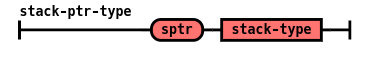
\includegraphics{nstar-stack-pointer-syntax}
  }
  \\
  \scalebox{.5}{
    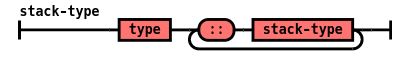
\includegraphics{nstar-stack-cons-syntax}
  }
  \caption{Grammar for stack types.}
  \label{fig:nstar-common-ts-stack-types-syntax}
\end{figure}

\subsection{Enumeration types}\label{subsec:nstar-common-ts-enums}

% TODO

\subsection{Structure types}\label{subsec:nstar-common-ts-structs}

% TODO

\subsection{Union types}\label{subsec:nstar-common-ts-unions}

% TODO

\section{File sections}\label{sec:nstar-common-sections}

Sections in N* serve the exact same purpose as in other assembly languages. They divide a file into multiple parts depending on what the semantics of the current section is supposed to be (code, data, etc).
Section names obviously differ from one target format to another. As an example, the ``\texttt{.rela.dyn}'' section from the ELF format may not exist in the PE format.

N* tries to unify target formats section names (simplifying targetting N* as a compiler backend) by having a fixed set of section names, all with different meanings. While you can put anything anywhere in classical assembly languages, this is not the case in N*.

Sections in N* can be named ``\texttt{data}'', ``\texttt{code}'' or ``\texttt{rodata}''. Each of them has defined semantics as described below.

\subsection{The \texttt{code} section}\label{subsec:nstar-common-sections-code}

The \texttt{code} section is the section containing all executable instructions (basically, as the name implies, code). Its syntax is defined in Figure~\ref{fig:nstar-common-sections-code-grammar}.

Each label is assigned a type, describing the context needed to branch to it.
If a label has the type \texttt{\{reg:s64\}} then there needs to be the register \texttt{reg} bound to a value of type \texttt{s64} in the current context, in order to branch to it.
However, some restrictions apply to labels in order to make the type-checking meaningful (or at least handle some aspects that cannot be handled with types only). See more about that in Section~\ref{sec:nstar-common-bs}~``\nameref{sec:nstar-common-bs}''.

\begin{figure}[htb]
  \centering
  \scalebox{.5}{
    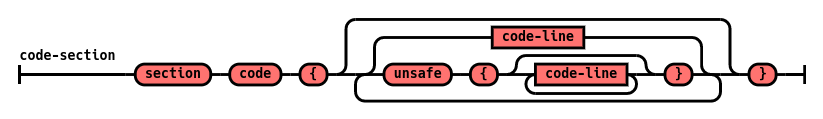
\includegraphics{nstar-code-section-1}
  }
  \\
  \scalebox{.5}{
    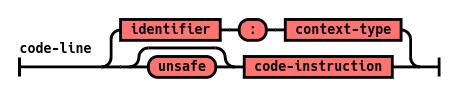
\includegraphics{nstar-code-section-2}
  }

  \caption{Grammar for \texttt{code} sections.}
  \label{fig:nstar-common-sections-code-grammar}
\end{figure}

Every assembly instruction makes the current context vary in some way, either by binding registers, forgetting about some bindings, changing register types, or some other way. The current context is just a record keeping track of the currently bound registers, along with the data type they contain. More on that in sections about instructions\footnote{Instructions are platform-specific, that's why we don't talk about them here.}.

\subsection{The \texttt{data} and \texttt{rodata} sections}\label{subsec:nstar-common-sections-data}

\section{Restrictions applied to branching}\label{sec:nstar-common-bs}

\section{Unsafe operations}\label{sec:nstar-common-unsafe}

\subsection{Dereferencing literal addresses}\label{subsec:nstar-common-unsafe-derefliteraladdr}

\subsection{Pointer offsetting}\label{subsec:nstar-common-unsafe-ptroffset}
